% ------------------------------------------------------------------------------------------------------------------------------------------------
\chapter{Analysis Job implementation results}
\label{chap:analysis-examples}

This chapter aims to provide tangible examples of how the previously described system works and in what way the parallel nature of the implemented system benefited these use cases.

The following two sections will focus on practical examples of so-called ''attacks'' (disortions) applied to the input media data, and how the proposed system has handled it. The examples have been selected to highlight the two major problems the system has to handle -- distorted image data and time shifted data.

In Section \ref{sec:mirrored-video-detection} video material will be analysed in order to find it's corresponding ''mirrored'' counter-part. This example will also be used to highlight the tremendous possibilities that lie within data \textit{pre-processing} that are applied within the proposed system, and if needed could be expanded even more in order to speed up the system's initial response time.

%In Section \ref{sec:scene-detection} an extracted scene will be positioned within an existing video in the reference database. This problem turns out to be non-trivial because of different frame-rates of supplied material, thus search methods similar, in concept, to sub-string search could not have been applied efficiently. The section explains the algorithms applied instead, and showcases an example case.

As this thesis is not focused on development of image analysis algorithms, these sections will instead lean their focus towards the distributed system and big-data parts of the problem. The image comparision algorithms also assume that that the used image correlation algorithm (\textit{phash} -- see Section \ref{sec:phash}) performs well enough for the job at hand. 

% -----------------------------------------------------------------------------------
\section{Near-duplicate video detection}
\label{sec:mirrored-video-detection}
In order to test the system in scenarios of image disortion the example case of ''mirrored'' video material was first used. This case is fairly popular among material uploaded to YouTube, so outside of the ease of preparing test data, it is also a valid real-life scenario of one might encounter -- content uploaders often ''flip'' the uploaded content in order to avoid copyright detection to trigger on content.

As will be shown in thie section, this ''attack'' is not very effective, as determining a exact-mirror video material is fairly simple. Even in the case of slight hue and luminescence changes the implemented system was able to detect such videos flawlessly.

\subsection{Analysed example material}
The material used to illustrate the this attack scenario originate from the movie ''\textit{Big Buck Bunny}'' \cite{big-buck-bunny} which has been created by the Blender Foundation \cite{blender-foundation} and released under the Creative Commons license \cite{creative-commons}. 

Figure \ref{fig:frames-mirrored} illustrates the original as well as mirrored counter part of an example frame taken from the movie. The analysed video material has been is in 1080p resolution. The entire movie was stored in the reference database in raw format, which amounts amounts to a total size of \verb|6.25GB|.


\begin{figure}[ch!]
        \centering
        \begin{subfigure}[b]{0.45\textwidth}
                
\includegraphics[width=\textwidth]{img/Big_Buck_Bunny_normal.png}
                \caption{Original frame}
                \label{fig:original-frame}
        \end{subfigure}
        \begin{subfigure}[b]{0.45\textwidth}
                
\includegraphics[width=\textwidth]{img/Big_Buck_Bunny_mirror.png}
                \caption{Mirrored frame}
                \label{fig:mirrored-frame}
        \end{subfigure}
        \caption{Example of original and mirrored frame}
        \label{fig:frames-mirrored}
\end{figure}





\subsection{Histogram calculation and HBase row key design}
The Map Reduce pipeline designed for detecting near-duplicate movies takes one very important fact into account: the histogram of an nearly identical movie will most likely not change very much. In the case of merely mirrored video material, the histogram will not change at all. This fact was utilised to design the row key for storing histograms in HBase for efficient lookup.

\begin{figure}[ch!]
  \centering
  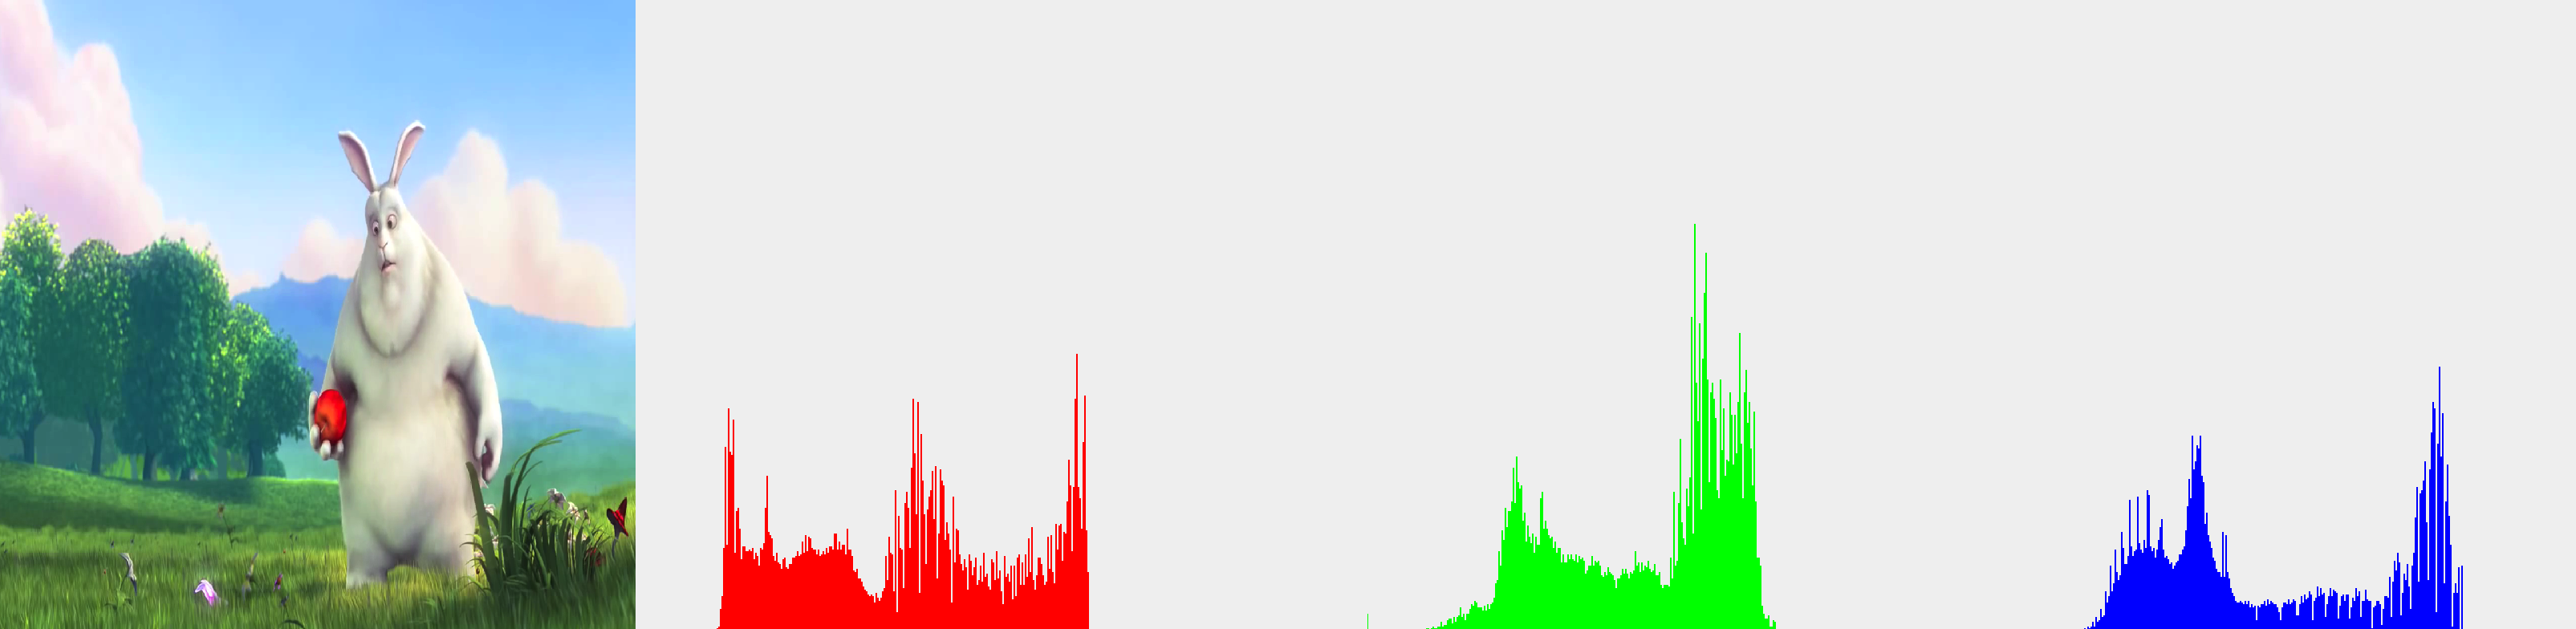
\includegraphics[width=\textwidth]{img/Histograms__Big_Buck_Bunny_mirror_png.png}
  \caption{R/G/B Histograms of analysed frame}
\end{figure}

Hbase's implementation provides strict guarantees about an HTables row key, specifically it guarantees to store data in \textit{alphabetically sorted order} based on it's row key. This property \textit{must} be taken into account when designing tables and keys in HBase. In particuilar it is a widely used technique to store parts of the data, or projections of it, directly in the key itself -- this is because HBase relies so much on the key to distribute data among RegionServers and a wrongly designed key may easily hot-spot one of the region servers (even in the presence of so called region-splitting, which re-shards the more work-intense regions onto multiple servers).

In our example, after obtaining the histogram data for each of the frames of an analysed movie, it is stored in the \verb|Histograms| table, with a precisely defined key. The key is designed to allow \textit{prefix queries} which are increadibly fast -- because HBase is able to determine, just by looking at the prefix query range, which exact RegionServers must be contacted, and they in turn are able to perform a linear scan of just the required region of the Table (which often means reading from disk). The key was designed using these guiding principles:

\begin{itemize}
 \item the key must allow for prefix queries, which given a ''to be compared frame'' will return ''probable candidates''
 \item more percise queries must also be possible to be constructed as prefix queries
\end{itemize}

Having this in mind, the key is designed to be an descending sorted \verb|-| joined list of color dominance in a given frame. Color dominance is calculated based on the percent of pixels in the image where one color's part would dominate (have a higher value) than any other color parts. For example given a pixel  \verb|RGB("#F2649D") = RGB(100, 242, 157)|, this pixel would be deemed to be \textit{green dominating}. 

\begin{lstlisting}[caption={Gramar for the Histogram RowKey. In essence, it contains an encoded color dominance value, the youtube id of the movie, and frame number.}, label={lst:row-key}]
    NUMBER           : [0-9]                              ;
    YT_ID            : .+                                 ; // youtube id
    FRAME            : NUMBER+                            ; // frame number
    COLOR            : ("R" | "G" | "B") NUMBER           ; // dominance of color in frame
    HIST_ORDERED : COLOR "-" COLOR "-" COLOR        ; // sorted by dominance

    ROW_KEY          : HIST_ORDERED ":" YT_ID ":" FRAME ;
    
    // examples: R57-B28-G13:YE7VzlLtp-4.mp4:22009  <- Red dominates
    //               G47-R41-G11:YE7VzlLtp-4.m6p4:919    <- Green dominates
\end{lstlisting}

Listing \ref{lst:row-ket} provides a simple ANTLR \footnote{ANTLR is a popular parser generator library for Java applications} gramar, which should make the key's parts easily visible (while ANTLR was not used directly for parsing of the key, it is a very clear and concise way of explaining the key's structure).

Having defined such key, Map Reduce jobs populate the reference database using it. Of course, the entire histograms would still be stored within the row (all 255 values for each color). The rest of the HTable's design is depicted on Figure \ref{fig:histogram-htable}.

This design allows the Analyser to issue very efficient queries for frames, such as in the examples shown in Table \ref{tab:scans}.

\begin{table}[ch!]
  \centering
  \begin{tabular}{|c|c|c|}
  \hline
  \textbf{Question}                  & \textbf{Query}                    & Prefix Scan \\ \hline
  Blue dominated frames              & \verb|START "B", END "B99"|       & Yes; Fast! \\ \hline
  Strongly red dominated frames      & \verb|START "R9", END "R99"|      & Yes; Fast! \\ \hline
  Green and Blue dominated frames (grass + sky) & \verb|FILTER "G*B*"|   & No; Slow \\ \hline
  All frames of Movie                & \verb|FILTER "*-e98uKex-*"|       & No; Slow \\ \hline
  \end{tabular}
  \caption{Examples of queries enabled by such RowKey design}
\end{table}

In the case of exact mirrored movies, it is possible to match the apropriate frames withing a few HBase queries, even before triggering the expensive Map Reduce Jobs, which force thousands of rows to be loaded. If this heurestic fails a full Map Reduce pipeline comparing frames by their perceptual hashes must be triggered.

\begin{figure}[ch!]
  \centering
  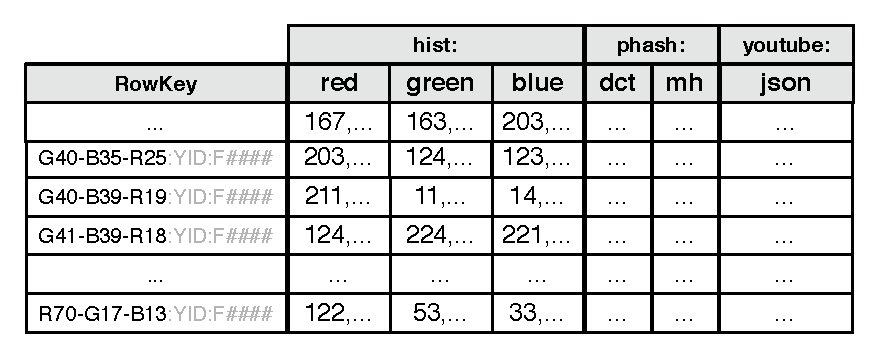
\includegraphics[width=\textwidth]{img/hbase-hashes-table}
  \caption{HBase HTable design used for histogram based lookups.}
  \label{fig:histogram-table}
\end{figure}


\begin{lstlisting}

REDUCER DOES:::::::


2014-05-07 00:49:51,225 INFO cascading.flow.hadoop.FlowReducer: sourcing from: GroupBy(_pipe_1*_pipe_2)[by:[{1}:'__groupAll__']]
2014-05-07 00:49:51,369 INFO cascading.flow.hadoop.FlowReducer: sinking to: Hfs["TextDelimited[['dctDist', 'histDist', 'mhDist', 'idRef', 'idAtt', 'frameRef', 'frameAtt']]"]["/oculus/compare-YE7VzlLtp-4_AND_e98uKex3hSw.out"]

234 map
1 reduce

Finished in: 44mins, 15sec

56,998,861,974 bytes produced
=======================

\end{lstlisting}




\newpage
\subsection{Role of perceptual hashing in near-duplicate detection}
\label{sec:perceptual-hashing}
Since simple histogram comparison if obviously not enough to determine if an image is of the same movie or not,
the second layer of comparison employed by the Analyser's Map Reduce Jobs is powered by perceptual hashing, as implemented by the phash \cite{phash} library.

As can be seen in Figure \ref{fig:histogram-table}, rows in the Histograms table contain not only the histogram values, but also the phash collumn family as well as youtube metadata. In this step of execution we will be comparing the already pre-filtered (by using the previous method) frames by their perceptual hashes. A detailed description and effectiveness analysis of these is available on the libraries website \footnote{PHash design and analysis -- http://www.phash.org/docs/design.html}.

During this work two perceptual hash implementations were used:
\begin{itemize}
  \item DCT hash -- Discrese Cosine Transform Hash; Is an efficient means to calculate an image hash based on it's
                    frequency spectrum data. It is usualy not sufficient in order to determine image similarity, 
                    but is a good accompanying hash function, which can be used in pair with other functions to increase 
                    their accuracy. If DCT does not match the given images, then most probably other algorithms also 
                    should not. It is also fairly efficient in detecting slight rotation and blurring. Experimentation 
                    conducted during this thesis show that a distance value lower than 20 points usually indicates a 
                    ''possible match'' using this algorithm.
                    
  \item MH hash -- based on the Marr--Hildreth algorithm \cite{marr-hildreth}, which is an edge detection algorithm.
                   The resulting ''hash value'' is in fact an compressed representation of the edges detected within the 
                   analysed image. This hash has a constant length of 72 bytes long hash, and can be comparef efficiently 
                   by using the classical Hamming Distance \cite{hamming-distance} method. This hashing algorithm is
                   usually sufficient to determing image equality. It is not very resilient against image rotation, but 
                   manages very well with blurring and differences in compared image resolutions. Used in pair with the 
                   DCT hash and histogram methods it is a very viable aproach to near-equality checks.
\end{itemize}

Listing \ref{lst:phashes-example} presets example hashes calculated for the frames seen in Figure \ref{fig:frames-mirrored}. It's worth pointing out that the dct hash in both cases is equal, while the mh hash is different changed - because it carries more information in it's 72 bytes.

\begin{lstlisting}[caption={Example hashes, calculated for a original and mirrored frame}, label={lst:phashes-example}]
// Big_Buck_Bunny_normal.png
dctHash = 54086765383280
mhHash  = 8e2f6d04831568425b3c5c2ca01afd88b6ad638d43ced55d71cc032c53a
            bdc898e930523e00fb334e765e57529f0ca5b6b6333a35076b1fd249a1e
            00e0e7c45beaa10792bc453228
                        
// Big_Buck_Bunny_mirror.png
dctHash = 54086765383280
mhHash  = 458193aa7ca2e2f03e29065f29f01019f4b813f07b217f94775dcb91985
            cc0ef83656b981b575f4d44ad7848c5469d1ad81a496665c3e262070e42
            4d8592231a1c8118fcf2f0ef63
\end{lstlisting}

Hashes like this can be compared to each other using a simple Hamming Distance \cite{hamming-distance} function, as their values at certain positions represent certain traits of the hashed picture. This is the core of the last phase of the matching algorithm. The Table \ref{tab:hash-distances} shows how the distance between these hashes differ in a few example scenarios. As is to be expected, the mh hash is reacting much more than the plain DCT hash. \todo{finish me}

\begin{table}[ch!]
  \centering
  \begin{tabular}{|c|c|c|}
    \hline 
    \textbf{Tested distortion}             & \textbf{DCT distance} & \textbf{MH distance} \\ \hline
    Mirrored frame                         & 0                     &  402 \\ \hline
    +20\% lumunosity                       & 0                     &  132 \\ \hline
    Blurring                               & 0                     &  246 \\ \hline
    Slightly different frames (next frame) & 25                    &  324 \\ \hline
    Different frames (moved character)     & 31                    &  355 \\ \hline
    
  \end{tabular}
  \caption{Example distances between sample frames, and their distorted versions.}
  \label{tab:hash-distances}
\end{table}



\subsection{Applicability in other video material distortion scenarios}

Of course, other kinds of disortions could be applied to a video, such as comparing a high-quality video with a low-quality counterpart or simple coloring filters. While being outside of the scope of this thesis, the basic concepts and framework proposed would easily be able to incorporate more scoring functions into the Map Reduce pipeline that would help determine matches between even such disorted video materials. 

An interesting example disortion found commonly in many materials is slight changes in the color hue or white balance of the \todo{histograms}.


% ------------------------------------------------------------------------------------------------------------------------------------------------
\section{Scene detection}
\label{sec:scene-detection}
This scenario can be explained as trying to find out \textit{where} (if at all) a scene takes place in a movie known to the reference database. 

Although on the sufrace the general problem statement is not so different than substring search, which is a known and well researched topic in computer science. In sub-string search algorithms like the Knuth–Morris–Pratt \cite{kmp-string-search} or the Boyer-Moore \cite{boyer-string-search} algorithms leverage that the ''matching'' either will apply, or will not in order to increase search speed in the worst case to still linear time. However, these methods can \textit{not} be directly applied to the problem specified in this section -- because of the dissortions in source and reference video material as well as the possibility of cross-matches when a movie is built up from multiple short scenes from other movies -- a typical example here would be ''flash-back'' scenes or ''top 10'' movies where before the last top-3, the movie would quickly go over already shown frames of scenes. Another problem adding to the dissortions is frame rates of reference data vs. an analysed video fragment -- even a slight missmatch (30FPS vs. 25FPS) would render the substring search algorithms not usable for this concrete example.

\begin{figure}[ch!]
  \centering
  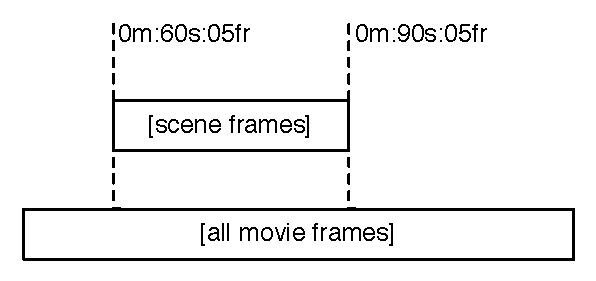
\includegraphics[width=0.6\textwidth]{img/frames-timeline-matching}
  \caption{Visual representation of the goal of this example application.}
\end{figure}

Instead, a more statistical aproach was taken. In which a frame is compared with it's set of ''potential match candidates'' which are determined by very coarse filtering of the reference data set by bucketing certain criteria of their histograms such as ''dominating red'' or ''dominating blue'' (this classification is prepared on the reference data beforehand -- during importing into the system).

\todo{mention somewhere before that we really extract data like ''mostly red''}

\todo{finish this scenario}

\begin{figure}[ch!]
  \centering
  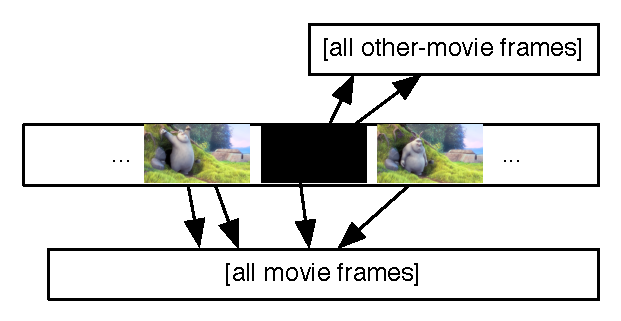
\includegraphics[width=0.6\textwidth]{img/frames-timeline-matching-missmatch}
  \caption{One frame may potentially match multiple reference frames. The final most probable matching scene is determined by aggregating data the direct frame-to-frame matches.}
\end{figure}



















